\chapter{Introducci\'on}

En Computer Graphics, la tecnica del shading permite mejorar la percepcion de
los volumenes en 3D. Con el aumento de la capacidad de computacion estas tenicas
han evolucionado mucho en un breve periodo de tiempo.\sidenote{Is this correct?}\sidenote{I'm unsure about also!}

Las primeras aportaciones el campo fueron durante los anhos 70 por parte de Bui
Tuong Phong, Henri Gouroud y Jim Blinn con sus modelos de shading: Phong\autocite{phong}, Gouraud\autocite{gouraud}
y Blinn-Phong\autocite{blinnphong}. Estos algoritmos permiten, a partir de la posicion de la luz, y la
position de la camara, dar una estimacion de la cantidad de luz emitida por una
superficie.
\singlespacing

\begin{figure}[H]
\setlength{\fboxsep}{0pt}
\fbox{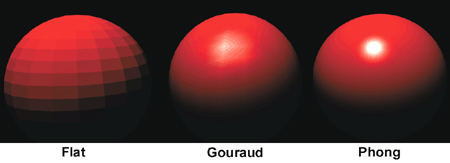
\includegraphics[width=0.99\linewidth]{images/gouroud-phong-flat.jpg}}
\caption{A boat.}
\singlespacing
\end{figure}

\todo[inline]{
    TODO: hablar sobre matriz de perspectiva de
    \href{http://www.cs.uns.edu.ar/cg/clasespdf/p465carlbom.pdf}
    {Ingrid Carlbon}
}

\todo[inline]{
    Siguientes a\~nos: antialising, sombras, multinucleo aparicion GPUs,
    raytracing...
    \href{https://ohiostate.pressbooks.pub/graphicshistory/back-matter/cg-historical-timeline/\#1970}
    {fuente}
}

\todo[inline]{
    Blinn’s law: “as technology advances, rendering time remains constant.” 
    from
    \href{http://www.pbr-book.org/3ed-2018/Introduction/A_Brief_History_of_Physically_Based_Rendering.html}
    {here}
}

\todo[inline]{
    Blinn's law: James Blinn first pointed out, in animation, rendering time remains
    constant, even as computers get faster. An artist gets accustomed to waiting a
    certain number of hours for an image to render, so as hardware improves, instead
    of using it to save time, he employs it to render more complex graphics. from
    \href{https://nevalalee.wordpress.com/2011/08/09/blinns-law-and-the-paradox-of-efficiency/}
    {here}
}

\todo[inline]{
    TODO: Esquema evolucion en el tiempo del shading: phong, blinn-phong
}

\todo[inline]{
    PBR, PBM, PBS

    Physically Based Rendering PBR is a method of shading and rendering that provides a more
    accurate representation of how light interacts with surfaces. It is referred to as Physically
    Based Rendering PBR or Physically Based Shading PBS. Depending on what aspect of the pipeline
    is being discussed, PBS is usually specific to shading concepts and PBR is specific to rendering
    and lighting. However, both terms describe the process of representing assets from a physically
    accurate standpoint.

    Physically based rendering PBR is an approach in computer graphics that seeks to render graphics
    in a way that more accurately models the flow of light in the real world. Many PBR pipelines have
    the accurate simulation of photorealism as their goal. Feasible and quick approximations of the
    bidirectional reflectance distribution function and rendering equation are of mathematical
    importance in this field. Photogrammetry may be used to help discover and encode accurate optical
    properties of materials. Shaders may be used to implement PBR principles.\\
    What are the benefits?

    As artists, we can view the benefits of PBR from an artistic and production efficiency mindset:

    1. PBR removes the guesswork of authoring surface attributes, such as specularity, since its methodology and algorithms are based on physically accurate formulas. It is therefore easier to create realistic-looking assets.
    2. Assets will look accurate in all lighting conditions.
    3. PBR provides a workflow for creating consistent artwork, even between different artists.
    
    Por primera vez en un paper de 1999 en la universidad de Cornell
}